\documentclass[12pt,letterpaper,noanswers]{exam}
\usepackage[usenames,dvipsnames,svgnames,table]{xcolor}
\usepackage[margin=0.9in]{geometry}
\renewcommand{\familydefault}{\sfdefault}
\usepackage{multicol}
\usepackage{wrapfig}
\pagestyle{head}
\header{AM 22b Class 31}{}{Apr 14: Differential equations, p.\thepage}
\runningheadrule
\headrule
\usepackage{graphicx} % more modern
\usepackage{amsmath} 
\usepackage{amssymb} 
\usepackage{hyperref}
\usepackage{tcolorbox}
\usepackage[utf8]{inputenc}
\usepackage{diagbox}
\usepackage{graphicx} 
\usepackage{enumitem}
\usepackage{tikz}
\tikzstyle{startstop} = [rectangle, rounded corners, minimum width=3cm, minimum height=1cm,text centered, draw=black]

\tikzstyle{process} = [rectangle, minimum width=3cm, minimum height=1cm, text centered, draw=black, fill=gray!20]
\tikzstyle{decision} = [ellipse, minimum width=3cm, minimum height=0.5cm, text centered, draw=black, fill=white!30]
\tikzstyle{arrow} = [thick,->,>=stealth]
\usetikzlibrary{shapes.geometric, arrows}
\pagenumbering{arabic}

\usepackage[numbered,autolinebreaks,useliterate]{mcode}

\newcommand{\mb}[1]{\underline{#1}}

\begin{document}
 \pdfpageheight 11in 
  \pdfpagewidth 8.5in




% I need to review the torus trajectories...

\begin{itemize}
% \item There is a pre-class assignment (20 minutes of videos + a few WeBWorK exercises) due at 10am this Monday.  It is available on Canvas.
\itemsep0em
\item There is a skill check Monday (C30, 31, 32).
\item Quiz 05 will be released this Friday.
\item Quiz 06 will be released next Friday.
\end{itemize}

\hrule
\vspace{0.2cm}

% partial derivatives, gradient
% local linearity, differential, directional deriv
% 2nd order partials + equations with partials

\noindent\textbf{Big picture}

We will learn how to analyze differential equations from three perspectives: using approximate solutions (slope fields + Euler's method + RK45), finding exact solutions (rarely, using separation of variables), using qualitative methods (identifying equilibrium solutions and whether they are `stable' or `unstable').

Today we will learn about the superposition property of solutions to some linear differential equations.  We will also construct a differential equation where solutions saturate.

\vspace{0.2cm}
\hrule
\vspace{0.2cm}

\noindent \textbf{Skill Check C31 Practice}

Show the mathematical steps to find a solution to $\frac{dx}{dt} = -4x, x(0) = 2$.

\vspace{0.2cm}
\hrule
\vspace{0.2cm}

\noindent \textbf{Skill Check C31 Practice Solution}

For the skill check, you'll need to show your mathematical steps but do not need to provide written descriptions of the steps.

\begin{enumerate}
    \item 'Separate' variables: $\frac{1}{x}\frac{dx}{dt} = -4$.
    \item Integrate both sides with respect to time.  $\displaystyle\int \frac{1}{x(t)}\frac{dx}{dt}dt = \int -4 dt$.
    \item Change variables on the left hand side: $u = x(t)$, 
    $du = \frac{dx}{dt}dt$.  
    $\int \frac{1}{u}du = -4t + C$
    \item Integrate the left hand side.  $\ln \vert u\vert = -4t + C$.
    \item Rearrange: $u = e^Ce^{-4t}$
    \item Return to the original variables: $x(t) = e^Ce^{-4t}$.
    \item Set $C$ so that $x(0) = 2$.  $x(0) = e^Ce^{0} = e^C = 2$.  $x(t) = 2e^{-4t}$. 
\end{enumerate}

\vspace{0.2cm}
\hrule
\vspace{0.2cm}

\noindent\textbf{Teams}

\begin{multicols}{2}

1.  student names
\end{multicols}


\vspace{0.2cm}
\hrule
\vspace{0.2cm}


%\noindent\textbf{Differential equations} \S 11.1

%A concept that I think could be confusing is the arbitrary constant after finding the solution to a differential equation. Ordinarily, after integrating, the arbitrary constant is added on. However, in this case, it's multiplied to the exponential term. I think about it this way: if a constant were added to the solution to a differential equation, then the derivative shouldn't change, but it does, since the y term in the derivative changed. Therefore, the arbitrary constant can't be added. However, if the constant C is multiplied by the exponential term, the derivative is likewise multiplied by the constant, and since, in the example, the "100" terms are cancelled out, the remaining value is also multiplied by the constant C. 

%One area I find potentially confusing is when solving a differential equation. The textbook uses the example of at what rate one learns new material, and the rate changes depending on how much the person knows. My slight confusion is in how often this is updated. For example, the textbook updates the rate of learning each day, so that at the end of each day, the rate at which the person will learn the next day is calculated. Could this not be done with any time interval though? If the rate truly is variable with knowledge, doesn't the rate change constantly, throughout each day, hour, almost constantly? I assume that the solution to this is just to choose a fixed time interval off of which to update the rate so as to increase simplicity.

%In the reading for the family of solutions, it says the horizontal solution curve when C=0 is called an equilibrium solution. Does every differential equation which has solutions have an equilibrium solution? What about those which only have a unique solution?

%I am confused about the family of solutions portion of the text, especially relating to the equilibrium solution. Does every differential equation have this solution? I am also struggling to interpret the meaning of the equilibrium solution, and why it would potentially be important.


\noindent\textbf{Differential equations}


\noindent\textbf{Example (population model)}

The population of the United States, $P$, has been measured every ten years since 1790 (via the decennial census).  (data in blue below)

We considered two different models:
\begin{enumerate}
    \item $\dfrac{dP}{dt} = a P$, or $\dfrac{dP/dt}{P} = a$ (red curves below: constant model for per capita population growth)
    \item $\dfrac{dP}{dt} = b P(1-P/K)$, or $\dfrac{dP/dt}{P} = b(1-P/K)$ (yellow curves below: linear model for per capita population growth)
\end{enumerate}

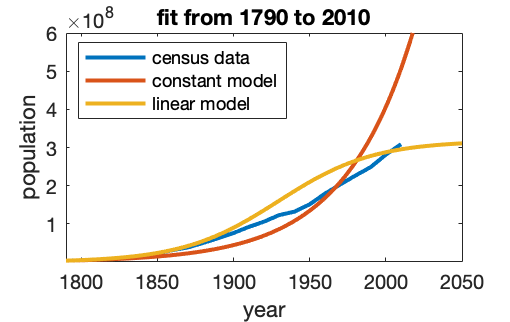
\includegraphics[width=0.33\linewidth]{img/C31p1b.png}
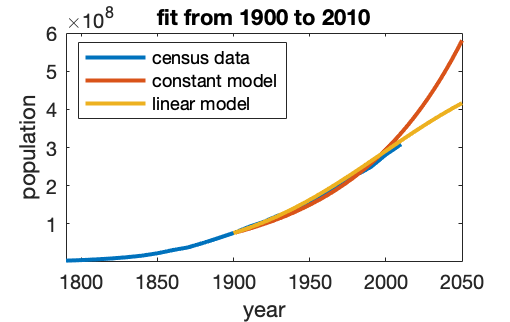
\includegraphics[width=0.33\linewidth]{img/C31p1c.png}
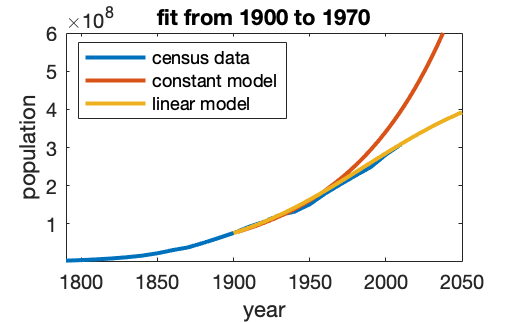
\includegraphics[width=0.33\linewidth]{img/C31p1a.png}

\noindent\textbf{Method}
\begin{enumerate}
    \item Approximate $\dfrac{dP/dt}{P}$ with $\dfrac{\Delta P/10}{P}$ from US Census data.
    \item Let $a$ be the mean value of $\dfrac{\Delta P/10}{P}$, averaged over the dataset.  Note: this is not the only way to fit this model to the data.
    \item Let $f(P) = b(1-P/K)$ be a line fit to the points $(P,\dfrac{\Delta P/10}{P})$.  Again there are other ways to choose the parameters to the model, but this is one way.
    \item Use Euler's method to find an approximate solution to $\dfrac{dP}{dt} = aP$, $P(0) =\text{US popn}(1790)$ and to $\dfrac{dP}{dt} = bP(1-P/K)$, $P(0) =\text{US population in}(1790)$, for $a,b,K$ as found above.
    \item Instead of using all of the data to find the line of fit, we might use a subset of the data instead.
    \begin{enumerate}
        \item (recent data) One way to subset is to only use more recent times (assume that the population growth mechanisms were different in 1790 from in 1900, but that 1900 or 1910 is reasonably similar to today).
        \item (fitting and test data)  Another way to subset is to reserve some recent data to ``test'' your model.  If you're interested in forward prediction of population, you could fit the model on data from 1900 to 1960 and then check the fit on data from 1970 to 2010.  By reserving some of the data, you're able to check how well your model `forecasted' into the future.
    \end{enumerate}
\end{enumerate}

\vspace{1in}

\eject
\vspace{0.2cm}
\hrule
\vspace{0.2cm}

\noindent\textbf{Exponential growth or decay}
\begin{tcolorbox}
\begin{itemize}
\itemsep0em
    \item The differential equation $\dfrac{dx}{dt} = ax$ has solutions of the form $x(t) = ke^{at}$.  
    \item For the \textbf{initial value problem}  $\dfrac{dx}{dt} = ax$ , $x(0) = x_0$, the solution is $x(t) = x_0e^{at}$.
    \item This differential equation can only encode exponential growth ($a>0$) or exponential decay ($a<0$) with time.  
\end{itemize}
\end{tcolorbox}
\noindent\textbf{Mathematical details}
\vspace{0.2cm}

Given $\dfrac{dx(t)}{dt} = ax(t)$, how do we find a solution to this differential equation?

Let $u = x(t)$.  $du = \dfrac{dx}{dt}dt$.  To integrate, $x(t)$ needs to be on the same side of the equation as $\frac{dx}{dt}$.
    
    
    \begin{align*}
        \displaystyle\int \frac{1}{x(t)}\dfrac{dx}{dt}dt = \int a dt &\Rightarrow \displaystyle\int \frac{1}{u}du = \int a dt\\
       &\Rightarrow \ln\vert u\vert = at + c \\
       &\Rightarrow u = ke^{at} \text{ with } k = e^c
    \end{align*}.
\vspace{0.2in}

\noindent\textbf{Common mistakes}
For $\frac{dx}{dt} = x$, common mistakes result in finding a solution of $xt+c$ or to $\frac{1}{2}x^2+c$.
\begin{itemize}
 \item What assumptions / procedures would lead to $xt+c$?  What is incorrect about them?
 \vspace{0.7in}
 
\item What assumptions / procedures would lead to $\frac{1}{2}x^2+c$?  What is incorrect about them?
\vspace{0.7in}
    \end{itemize}
    
    
\noindent\textbf{Avoiding common mistakes}

When you find a solution to a differential equation, writing the solution in the form $x(t) = ...$ can help you see whether it makes sense.  Specifically, writing $x(t)$ every time there is an $x$, can remind you that $x$ and $t$ are linked together, rather than independent.

\vspace{0.5in}


\vspace{0.2cm}
\hrule
\vspace{0.2cm}

% \noindent\textbf{Exponential growth vs logistic growth}

% \noindent\textbf{Example.  Exponential growth.} Consider the population model $\frac{dP}{dt} = kP$.  Identify the range of $P$ for which $\frac{dP}{dt}$ is positive, negative, or zero.
% \vspace{1in}

% \noindent\textbf{Example.  Logistic growth.} Consider the population model $\frac{dP}{dt} = kP(b - P)$.  Identify the range of $P$ for which $\frac{dP}{dt}$ is positive, negative, or zero.
% \vspace{1in}

% \noindent\textbf{Stability of an equilibrium solution}
% \begin{tcolorbox}
% \begin{itemize}
% \itemsep0em
%     \item 
% \end{itemize}
% \end{tcolorbox}


\eject



\noindent\textbf{Superposition: Is the sum of two solutions also a solution?}
\begin{tcolorbox}
\begin{itemize}
\itemsep0em
    \item A \textbf{linear differential equation} is a differential equation of the form $f(x,\frac{dx}{dt}, \frac{d^2x}{dt^2}, ...) = 0$ where $f$ is a linear polynomial in $x$ and its derivatives.
    \begin{itemize}
        \itemsep0em
        \item Example: $\dfrac{d^2x}{dt^2} + 2\cos t \frac{dx}{dt} - 3t^3 x = 0$ is linear differential equation.
   \item  Non-example: $\dfrac{d^2x}{dt^2} + 2\cos t \frac{dx}{dt}x - 3t^3 x = 0$ is nonlinear differential equation.
    \end{itemize}
    \item A linear differential equation is called \textbf{homogeneous} when there are no constant terms in the equation.  
    \begin{itemize}
    \itemsep0em
        \item Example: $\dfrac{dx}{dt} - 3x = 0$ is homogeneous. 
   \item  Non-example: $\dfrac{dx}{dt} - 3x + 2 = 0$ is nonhomogeneous.
    \end{itemize}
\end{itemize}

\end{tcolorbox}

\noindent\textbf{Example: addition of solutions}.  

$\dfrac{dx}{dt} - t x = 0$ is a linear homogeneous differential equation.  Assume $x_1(t)$ is a solution of this equation.  Assume $x_2(t)$ is a solution as well.  Consider $x_3(t) = a_1x_1(t) + a_2x_2(t)$ for $a_1$ and $a_2$ constants.  Show that $x_3(t)$ is a solution of the differential equation.
\begin{enumerate}
    \item Given that $x_1(t)$ and $x_2(t)$ are solutions, write out mathematical statements satisfied by $x_1(t)$ and by $x_2(t)$.  \emph{Do not attempt to find $x_1(t)$ or $x_2(t)$ in closed form (i.e. don't try to solve the equation), instead, use that fact that they are solutions to find mathematical statements that they must satisfy.}
    \vspace{1in}
    
    \item Use the statements you've written above to show that $\dfrac{d x_3}{dt} - t x_3 = 0$.
    \vspace{1in}
\end{enumerate}

\noindent\textbf{Example: no addition of solutions}.
$\dfrac{dx}{dt} - t x + 2 = 0$ is a linear nonhomogeneous differential equation.  Assume $x_1(t)$ is a solution of this equation.  Assume $x_2(t)$ is a solution as well.  Consider $x_3(t) = a_1x_1(t) + a_2x_2(t)$ for $a_1$ and $a_2$ constants.  How does the argument you used above break down when you try to show that $x_3(t)$ is a solution?
\vspace{2in}

\noindent\textbf{Example: no addition of solutions}.
$\dfrac{dx}{dt} - t x^2 = 0$ is a nonlinear differential equation.  Assume $x_1(t)$ is a solution of this equation.  Assume $x_2(t)$ is a solution as well.  Consider $x_3(t) = a_1x_1(t) + a_2x_2(t)$ for $a_1$ and $a_2$ constants.  How does the argument you used above break down when you try to show that $x_3(t)$ is a solution?
\vspace{2in}

\noindent\textbf{The principle of superposition}
\begin{tcolorbox}
If $x_1(t)$ and $x_2(t)$ are two solutions to a linear, homogeneous, differential equation, then $x(t) = a_1 x_1(t) + a_2x_2(t)$ is also a solution.  This is called the principle of \textbf{superposition}.
\end{tcolorbox}

\eject

\vspace{0.2cm}
\hrule
\vspace{0.2cm}



% \noindent\textbf{Growth that saturates}
% \begin{tcolorbox}
% \begin{itemize}
% \itemsep0em
%     \item We say that a solution \textbf{saturates} when $x(t) \rightarrow k$ as $t\rightarrow \infty$ (so the solution approaches a constant as time increases).
%     \item Assume $x(t)$ is an increasing function of time.  For the function to approach a constant, $k$, its rate of increase must approach zero as $x$ nears $k$.
%     \item Solutions of $\frac{dx}{dt} = ax$ cannot saturate.
%     \item To add saturation, consider $\dfrac{dx}{dt} = ax - bx^2$.
% \end{itemize}
% \end{tcolorbox}




% \noindent\textbf{Equilibrium solutions}

% Find the equilibrium solutions of $\dfrac{dx}{dt} = ax - bx^2$.

% \vspace{1in}

% \noindent\textbf{Matlab interlude}

% Head to Matlab and use the provided code to make a slope field.  
% \begin{enumerate}
%     \item Vary $a$ and $b$.  How does changing each of them alter your slope field?
%     \vspace{1in}

%     \item Based on the slope field, describe the shape of solutions to this differential equation.  At what value do solutions saturate?
% \end{enumerate}


% We will approximate solutions of a differential equation near an equilibrium solution.

% \vspace{0.2cm}
% \hrule
% \vspace{0.2cm}
\noindent\textbf{Approximating solutions near an equilibrium}
\begin{tcolorbox}
\begin{itemize}
\itemsep0em
\item We found an exact solution, $x(t) = x_0e^{at}$ to the initial value problem $\dfrac{dx}{dt} = ax$, $x(0) = x_0$.  For other differential equations, given an initial conditions near an equilibrium solution, we will be able to approximate the solution via this linear differential equation.
    \item Consider a differential equation $\dfrac{dx}{dt} = f(x)$.  At equilibrium solutions, $x(t) = x^*$.  For $x(0) - x^*$ small, we approximate the differential equation by Taylor expanding.
    \item Taylor expand $f(x)$ about the equilibrium solution.  Doing this, and solving the resulting (approximate) differential equation, we find $x(t) \approx x^* + (x(0)-x^*)e^{ct}$ where $c = \left.\frac{df}{dx}\right\vert_{x^*}$.
    \item You can think of a solution $x(t)$ to a nonlinear differential equation $\frac{dx}{dt} = f(x)$ as a combination of exponential growth away from an equilibrium where $f'(x^*)>0$ and exponential decay towards an equilibrium where $f'(x^*)<0$.
    \item We call an equilibrium solution \textbf{stable} if nearby solutions decay towards it ($f'(x^*)<0$).  We call it \textbf{unstable} if nearby solutions grow away from it ($f'(x^*)>0$).  \emph{We leave the $f'(x^*) = 0$ case alone for now}.
\end{itemize}
\end{tcolorbox}
\noindent\textbf{Mathematical details}

     To approximate solutions to $\dfrac{dx}{dt} = f(x)$ near an equilibrium solution, $x(t) = x^*$, notice that $\frac{dx}{dt}\approx f(x^*) + (x-x^*)f'(x^*)$ (Taylor expansion).  At an equilibrium, $x^*$, we have $f(x^*) = 0$.  In addition, $c = f'(x^*)$ is a constant, so this becomes $\dfrac{dx}{dt} \approx c(x-x^*)$.
     
     Notice that $\frac{d(x-x^*)}{dt} = \frac{dx}{dt}$ so we have $\frac{d(x-x^*)}{dt}\approx c(x-x^*)$.  Near $x^*$, $x-x^* \approx ke^{ct}$ where $k = x(0) -x^*$.  So we have $x(t) \approx x^* + (x(0)-x^*)e^{ct}$.
     \vspace{2in}
     
     \noindent\textbf{Example}
     Classify the equilibrium solutions of $\frac{dx}{dt} = ax - bx^2$, with $a,b>0$ as stable or unstable.
     \vfill
    
    \vspace{0.2cm}
\hrule
\vspace{0.2cm}

\end{document}